%\documentclass[a4paper,twoside,10pt,openright]{report}%Dokumentenklasse 
\usepackage{graphicx} %Compiler

\usepackage{dsfont}

%%%% Schrift und Kodierung %%%%
	\usepackage[T1]{fontenc} %Zeichensatzkodierung von 7bit auf 8bit 
	\usepackage[utf8]{inputenc} %Zeichensatzkodierung Unicode bzw. UTF8
	\usepackage{lmodern} %Vektorschrift
	%\RequirePackage[english,spanish,es-nolayout]{babel}
	\usepackage[english]{babel}
	\usepackage{textcomp}
	\usepackage{lmodern}
	\usepackage{url}
	\usepackage[bookmarksnumbered=true]{hyperref}
    \graphicspath{{figures/}}	
	
%%% COLORS %%%
\newcommand{\hl}[1]{
   \textcolor{MidnightBlue!90!black}{#1} 
}

\usepackage{pifont}% http://ctan.org/pkg/pifont
\newcommand{\cmark}{\ding{51}}%
\newcommand{\xmark}{\ding{55}}%

\usepackage{stackrel}

\usepackage{feynmp}

\usepackage{amsthm}
\newtheorem{definition}{Definition}
\newtheorem{proposition}{Proposition}
	
%%%% Fancy Header %%%
\usepackage{fancyhdr}
\usepackage[dvipsnames]{xcolor}
\usepackage{tikz} 
\usepackage{pgfplots}
%\usepackage{pgf-pie}

\usetikzlibrary{arrows}
\usetikzlibrary{shapes.geometric, arrows}

\definecolor{mycolor}{rgb}{0.45,0.45,0.45}% dark grey

\newcommand{\mcD}{\mathcal{D}}
\newcommand{\mcL}{\mathcal{L}}
\newcommand{\dth}{\Delta_{\text{th/sys}}}
\newcommand{\dst}{\Delta_{\text{stat}}}
\newcommand{\dsy}{\Delta_{\text{syst}}}
\newcommand{\sthsy}{\sigma_{\text{th/sys}}}
\newcommand{\sth}{\sigma_{\text{th}}}
\newcommand{\sst}{\sigma_{\text{stat}}}
\newcommand{\ssy}{\sigma_{\text{syst}}}

\newcommand{\Langle}{\big\langle}
\newcommand{\Rangle}{\big\rangle} 
 
\fancyhf{}
\fancyhead[LE]{\sffamily\color{mycolor}\nouppercase{\leftmark}} % left even, right odd
\fancyhead[RO]{\sffamily\color{mycolor}\nouppercase{\rightmark}} % left even, right odd
\fancyfoot[CE,CO]{\sffamily\color{mycolor}\nouppercase{\thepage}} % center even, center odd
\renewcommand{\headrule}{{\color{mycolor}%
\hrule width\headwidth height\headrulewidth \vskip-\headrulewidth}}
\renewcommand{\headrulewidth}{0.5pt}

\fancypagestyle{plain}{%
    \fancyhf{}%
    \fancyfoot[CE,CO]{ { \sffamily\color{mycolor}{\thepage} } }
	\renewcommand{\headrulewidth}{0.0pt}
}

%\fancypagestyle{fancy}{%
%   \fancyhf{}
%	\fancyhead[LE,RO]{\sffamily\color{mycolor}\nouppercase{\leftmark}} % left even, right odd
%	\fancyfoot[CE,CO]{\sffamily\color{mycolor}\nouppercase{\thepage}} % center even, center odd
%	\renewcommand{\headrule}{{\color{mycolor}%
%	\hrule width\headwidth height\headrulewidth \vskip-\headrulewidth}}
%	\renewcommand{\headrulewidth}{0.5pt}
%}


%%% Customize titles %%%%
\usepackage[ ]{titlesec}  %
\usepackage{etoolbox}
\makeatletter
\patchcmd{\ttlh@hang}{\parindent\z@}{\parindent\z@\leavevmode}{}{}
\patchcmd{\ttlh@hang}{\noindent}{}{}{}
\makeatother
%\titleformat{\chapter}[display]
%  { \normalsize \huge  \color{black}}%
%  {\flushright \normalsize \color{mycolor} \MakeUppercase %
%  {\sffamily \chaptertitlename } \hspace{1 ex}%
%  { \fontsize{60}{60}\selectfont \color{mycolor} \sffamily  \thechapter }}%
%  {10 pt}%
%  {\sffamily \huge \color{mycolor}\bfseries}
%\newcommand\mychapformat[1]{\parbox[t]{\dimexpr\textwidth-3em\relax}{\raggedleft#1}}
\titleformat{\chapter}[hang]{\Huge\bfseries\color{mycolor}\sffamily}% the number
	{\thechapter\hspace{20pt}\textcolor{mycolor}{|}\hspace{20pt}}%
	{0pt}{\Huge\bfseries\color{mycolor}\sffamily}% the title
\titleformat*{\section}{\sffamily\LARGE\color{mycolor}}
\titleformat*{\subsection}{\sffamily\Large\color{mycolor}}
\titleformat*{\subsubsection}{\sffamily\large\color{mycolor}}
\titleformat*{\paragraph}{\sffamily\large\bfseries\color{mycolor}}



	
%%%% Mathepakete %%%%
	\usepackage{array}
	\usepackage{calc}
	\usepackage{amsmath}
	\usepackage[intlimits]{empheq}
	\usepackage{amssymb,mathrsfs}
	\usepackage{theorem}
	\usepackage{slashed}
	\usepackage{feynmp-auto}

%%%% Sonstiges %%%%
	%\usepackage{subcaption}
	\expandafter\def\csname ver@subfig.sty\endcsname{}
	\usepackage{subfig} %Ermöglicht subfloats, also mehrere Tabellen/Bilder in einer Umgebung
	\usepackage{float} %Setzt mit [H] Figuren genau dort hin, wo sie im Text auftauchen
	\usepackage{booktabs} %Andere Tabellen
	\usepackage{gensymb}
	\usepackage{extarrows}%lange Pfeile
%	\usepackage{pst-pdf}	
	\usepackage{wasysym} %Symbolpaket
	\usepackage{multirow} %Ein Wert für mehrere Zeilen oder Spalten von Tabellen. Verwendung \multirow{#AnzahlZeilen}{*}{Name} bzw. analog \multicolumn{}{}{}
	\usepackage{rotating} %ermöglicht Schiefe Schrift
	%\usepackage{ziffer} %Deutsche Zahlen (Komma als Dezimalstelle im Mathemodus!)
	\usepackage{nicefrac} %Im Text schöne Brüche
	\usepackage[inner=3cm, outer=2.4cm, top=3cm]{geometry} %Passt Seitenränder an (left, right, top, bottom, width, height, textwidth, textheight)
	\usepackage{scrhack} %Verbessert angeblich LaTeX-Pakete
	\usepackage{numprint} %ROOT-Zahlen in deutsches zahlenformat übertragen. Syntax: \numprint[kg]{1.234e56} wird zu 1,234 * 10^56 kg
	\usepackage{cite}
	\usepackage{placeins}
	\usepackage{changepage}
	%\hyphenation{con-fine-ment}
	
%%%% spezielle Formatierungen %%%%
	\setlength{\emergencystretch}{25pt} %verhindert das Herausragen von Wörtern übers Zeilenende
	\setlength{\parindent}{0pt} %Kein Einschub bei neuem Absatz
	\setlength{\parskip}{2pt plus 1pt} %Erhöht Abstand zwischen Absätzen (um 1pt flexibel bei Seitenumbrüchen)
	
	%%%% Dokument-Variablen %%%%
\date{\today}

%%%% Eigene Befehle %%%%
\DeclareGraphicsRule{*}{mps}{*}{}
	\newcommand{\mE}[1]{\,\mathrm{#1}} %Einheiten im Mathemodus
	\renewcommand{\sl}[1]{\slashed{#1}} %Feynman-Slash
	\newcommand{\dummyImage}[2]{  %Erzeugt eine Umgebung wie includegraphics
		\frame{\mbox{\rule{0pt}{#2}	Bild fehlt  noch \rule{#1}{0pt}}}
	}
	\renewcommand{\i}{\mathrm{i}} %Imaginäre Einheit
%	\renewcommand{\vec}[1]{\textbf{#1}} %Fette Vektoren
	\newcommand{\bc}{\begin{center}}
	\newcommand{\ec}{\end{center}}

\newcommand{\matM}{\mathcal{M}}
\newcommand{\matH}{\mathcal{H}}
\newcommand{\matS}{\mathcal{S}}
\newcommand{\matU}{\mathcal{U}}
\newcommand{\matUL}{\mathcal{U}_L}
\newcommand{\matUR}{\mathcal{U}_R}

%%% center all the figures and tables
\makeatletter
\g@addto@macro\@floatboxreset\centering
\makeatother

%% maximal number of floating environments on each page 
\setlength{\floatsep}{0pt}
\setcounter{topnumber}{1}
\setcounter{bottomnumber}{1}
\setcounter{totalnumber}{1}
\renewcommand{\topfraction}{1.0}
\renewcommand{\bottomfraction}{1.0}
\renewcommand{\textfraction}{0.0}
\renewcommand{\thefootnote}{\fnsymbol{footnote}}

\def\tablename{Table}
\def\figurename{Figure}

\newcommand{\newparagraph}{\par\bigskip\noindent}
\newcommand{\toolfont}[1]{\texttt{#1}}
\newcommand{\ord}{\ensuremath{\mathcal{O}}}
\newcommand{\ope}[1]{\ensuremath{\mathcal{O}_{#1}}}
\newcommand{\largex}{\ensuremath{\large \boldsymbol{\times}}}
\newcommand{\brlargex}{\ensuremath{\large (\boldsymbol{\times})}}
\newcommand{\mheavy}{\ensuremath{M}}

\newcommand{\lag}{\ensuremath{\mathcal{L}}}
\newcommand{\mat}{\ensuremath{\mathcal{M}}}
\newcommand{\delx}{\ensuremath{\Delta}}
\newcommand{\data}{\ensuremath{\mathcal{D}}}
\newcommand{\jump}{\vspace{0.3cm}}
\newcommand{\bsg}{\ensuremath{\mathcal{B}(b \to s \gamma)}}
\newcommand{\rself}{\ensuremath{\hat{\Sigma}}}
\newcommand{\retildehat}{\ensuremath{\mbox{Re}\hat{\Sigma}}}
\newcommand{\retilde}{\ensuremath{\mbox{Re}\,\Sigma}}
\newcommand{\dweaksing}{\ensuremath{\delta_{\text{weak}}^{\text{sing}}}}
\newcommand{\dweak}{\ensuremath{\delta_{\text{weak}}}}
\newcommand{\newtext}[1]{\textcolor{red}{#1}}
\newcommand{\suit}{\textcolor{blue}{$\spadesuit$}}
\newcommand{\neutn}{\ensuremath{\tilde{\chi}^0_n}}
\newcommand{\gluino}{\ensuremath{\tilde{g}}}
\newcommand{\squark}{\ensuremath{\tilde{q}}}
\newcommand{\met}{\ensuremath{\slashed{E}_T}}
\newcommand{\nqsq}{\ensuremath{\tilde{\chi}\,\tilde{q}\,q}}
\newcommand{\msbar}{\ensuremath{\overline{MS}}}
\newcommand{\sw}{\ensuremath{s_w}}
\newcommand{\swd}{\ensuremath{s^2_w}}
\newcommand{\cw}{\ensuremath{c_w}}
\newcommand{\cwd}{\ensuremath{c^2_w}}
\newcommand{\myrbox}[1]{\parbox{4.0cm}{#1}}

\usepackage{xspace}
\newcommand{\brinv}{\ensuremath{BR_{\text{inv}}}\xspace}
\newcommand{\vegas}{\textsc{Vegas}\xspace}
\newcommand{\madgraph}{\textsc{Madgraph}\xspace}
\newcommand{\geant}{\textsc{Geant4}\xspace}
\newcommand{\pythia}{\textsc{Pythia}8\xspace}
\newcommand{\fastjet}{\textsc{FastJet}\xspace}
\newcommand{\delphes}{\textsc{Delphes}\xspace}
\newcommand{\sherpa}{\textsc{Sherpa}\xspace}
\newcommand{\sklearn}{\textsc{scikit-learn}\xspace}
\newcommand{\keras}{\textsc{Keras}\xspace}
\newcommand{\tensorflow}{\textsc{TensorFlow}\xspace}
\newcommand{\pytorch}{\textsc{PyTorch}\xspace}
\newcommand{\theano}{\textsc{Theano}\xspace}
\newcommand{\adam}{\textsc{Adam}\xspace}

\newcommand{\psib}{\overline{\psi}}
\newcommand{\bpm}{\begin{pmatrix}}
\newcommand{\epm}{\end{pmatrix}}

\newcommand{\p}{\partial}
\newcommand{\br}{\text{BR}}
\newcommand{\qqquad}{\qquad \qquad}
\newcommand{\qqqquad}{\qquad \qquad \qquad}

\newcommand{\matx}{|\mathcal{M}|^2}
\newcommand{\really}{\stackrel{!}{=}}
\newcommand{\SFitter}{\textsc{SFitter} }

% units of measure
\newcommand{\mev}{{\ensuremath\rm MeV}}
\newcommand{\gev}{{\ensuremath\rm GeV}}
\newcommand{\tev}{{\ensuremath\rm TeV}}
\newcommand{\fb}{{\ensuremath\rm fb}}
\newcommand{\ab}{{\ensuremath\rm ab}}
\newcommand{\pb}{{\ensuremath\rm pb}}
\newcommand{\sign}{{\ensuremath\rm sign}}
\newcommand{\iab}{\text{ab}^{-1}}
\newcommand{\ifb}{{\ensuremath\rm fb^{-1}}}
\newcommand{\ipb}{{\ensuremath\rm pb^{-1}}}

% really great macro by Chris Lester
\def\slashchar#1{\setbox0=\hbox{$#1$}           % set a box for #1
   \dimen0=\wd0                                 % and get its size
   \setbox1=\hbox{/} \dimen1=\wd1               % get size of /
   \ifdim\dimen0>\dimen1                        % #1 is bigger
      \rlap{\hbox to \dimen0{\hfil/\hfil}}      % so center / in box
      #1                                        % and print #1
   \else                                        % / is bigger
      \rlap{\hbox to \dimen1{\hfil$#1$\hfil}}   % so center #1
      /                                         % and print /
   \fi}
\newcommand{\dslash}{\slashchar{\partial}}
\newcommand{\Dslash}{\slashchar{D}}

\def\eg{{e.g.}\ }
\def\ie{{i.e.}\ }
%\def\etal{{\sl et al} \,}
%\DeclareMathOperator{\tr}{Tr}
\newcommand{\pbp}{\ensuremath{H^\dagger\,H}}
\DeclareMathOperator{\tr}{Tr}
\newcommand{\Dfb}{\mbox{$\raisebox{2mm}{\boldmath ${}^\leftrightarrow$}\hspace{-4mm} D$}}
\newcommand{\Dfba}{\mbox{$\raisebox{2mm}{\boldmath ${}^\leftrightarrow$}\hspace{-4mm} D^a$}}
\newcommand{\overbar}[1]{\mkern 1.5mu\overline{\mkern-1.5mu#1\mkern-1.5mu}\mkern 1.5mu}
\let\vec\mathbf % vectors in bold
\renewcommand{\d}{\text{d}}


%\pagestyle{fancy}
%\graphicspath{{../figures/}}	
%\begin{document}

\chapter[What is the uncertainty of generative models?]{What is the uncertainty of\\ generative models?}\label{chap:bnn}

\enlargethispage{2ex}
\vspace*{-2pt}

\enlargethispage{2ex}

{\bf Following the growing interest in refining LHC simulations with deep generative models, a crucial question to realistically use them in an analysis, is how to define and estimate the uncertainty associated to models output. 
We illustrate how approximate Bayesian inference can be used to define an uncertainty over a generative model's output.
Our findings show a highly non-trivial pattern in the model uncertainty, which may be understood in terms of a functional fit of the learnt density.}

%%%%%%%%%%%%%%%%%%%%%%%%%%%%%%%%%%%%%%%%%%%%%%%%%%%%%%%%%%%%%%%%%%%%%%%%
\section{Introduction}
\label{sec:binnintro}

In Chap.~\ref{chap:unfolding} we have shown that deep generative models certainly
possess the expressive power that we need to produce realistic synthetic data.
However, expressive power is not the only feature needed for their realistic use
in particle physics analysis. When data is simulated via standard Monte Carlo methods,
there's a clear understanding of what is the associated statistical error. 

Assuming a simple set-up in which we wish to estimate the observable
\begin{align}
\mathcal{O} = \int_x ~ dx f(x),
\end{align}
we can estimate $\mathcal{O}$ via Monte Carlo
\begin{align}
\mathbb{E}\left[\mathcal{O}\right] = \frac{1}{N} \sum_{i=1}^N f(x_i)
\end{align}
with uncertainty
\begin{align}
\text{Var}\left[\mathbb{E}\left[\mathcal{O}\right] \right] = \frac{\text{Var}\left[ f(x)\right]}{N}.
\end{align}
It is not within the scope of this chapter to discuss standard methods such as optimized
importance sampling to improve the standard integration described above, instead, we
want emphasize that as $\mathcal{O}$ is estimated using the "true" function $f(x)$, the 
only relevant figure is the number of samples $N$.
This is clearly not the case for approaches like the one described in Ref.~\cite{gan_phasespace},
where a generative model completely replaces the integrator.
As generative models only approximates a desired distribution, in this case the 
integrand $f(x)$, they should be used with caution if and when precision is required.
In other worlds, if an additional rejection sampling based on the truth is not added on top
of the generative model, our prediction will also include uncertainties from the fact
that we generate samples from some function $\tilde{f} \sim f$, and this extra uncertainty
collects everything associated to model's training.
This does not mean that such an approach should be discarded entirely, but rather
that we should think of a way to estimate this approximation uncertainty.

The fact that experiments, field theory calculations, and simulations
control their uncertainties implies that we can work with a complete
uncertainty budget, including statistical, systematic, and theory
uncertainties. To sustain this approach at the upcoming HL-LHC, with a
data set more than 25 times the current Run~2 data set, the
challenge is to provide faster simulations while keeping full control of
the uncertainties.

In recent years it has been shown that modern machine learning can
improve LHC event simulations in various ways. 
Promising techniques include deep generative models such as generative 
adversarial networks
(GAN)~\cite{goodfellow,Creswell2018}, variational 
autoencoders~\cite{kingma2014autoencoding,Kingma2019}, and
invertible models~\cite{nflow1,nflow_review,papamakarios2019normalizing,nflow_review,mller2018neural, inn,coupling2,glow}. 
%They can improve phase space integration~\cite{maxim,Chen:2020nfb}, phase
%space sampling~\cite{Bothmann:2020ywa,Gao:2020vdv,Gao:2020zvv}, and
%amplitude computations~\cite{Bishara:2019iwh,Badger:2020uow}.  
Further developments are fully NN-based event generation~\cite{dutch,gan_datasets,DijetGAN2,gan_phasespace,Alanazi:2020klf}, detector
simulation~\cite{calogan1,calogan2,fast_accurate,aachen_wgan1,aachen_wgan2,ATLASShowerGAN,ATLASsimGAN,Belayneh:2019vyx,Buhmann:2020pmy,Buhmann:2021lxj},
or parton showering~\cite{shower,by_example,monkshower,juniprshower,Dohi:2020eda}.
Generative models may also improve searches for physics beyond the
Standard Model~\cite{bsm_gan}, anomaly
detection~\cite{Nachman:2020lpy,Knapp:2020dde}, detector
resolution~\cite{DiBello:2020bas,Baldi:2020hjm}, and
inference~\cite{Brehmer:2020vwc,radev2020bayesflow}. Finally,
conditional GANs and INNs allow us to invert the simulation chain to
unfold detector effects~\cite{Datta:2018mwd,fcgan} and extract the
hard scattering process at parton level~\cite{Bellagente:2020piv}. The
problem with these applications is that little is known about
%
\begin{enumerate}
\item how these generative networks work, and
\item what the uncertainty on the generative network output is.
\end{enumerate}
%
As we will see in this chapter, these two questions may be related.

In general, we can track statistical uncertainties in
neural network outputs with Bayesian
networks~\cite{bnn_early,bnn_early2,bnn_early3,deep_errors}. Such
networks have been used in particle physics for a long
time~\cite{bnn_tev,bnn_tev2,bnn_Nu}. For the LHC we have proposed to
use them to extract uncertainties in jet
classification~\cite{Bollweg:2019skg} and jet
calibration~\cite{Kasieczka:2020vlh}. 
They can cover uncertainties related to statistical and structural
limitations of the training sample~\cite{Nachman:2019dol}, while being obviously unable to track
systematic uncertainties.  Similar ideas can be used as part of ensemble techniques~\cite{Araz:2021wqm}.
We propose to use a Bayesian INN (BINN) to extract uncertainties induced by the network training on a
generated event sample.

Because invertible models allows to evaluate the likelihood exactly, 
they are a natural tool for evaluating the uncertainty over the learnt
distribution, compared to implicit models like generative adversarial networks.
While Bayesian classification~\cite{Bollweg:2019skg} and regression
networks~\cite{Kasieczka:2020vlh} highlight the statistical and
nature of uncertainties, our Bayesian generative network
exhibits a very different structure. We will discuss the learning
pattern of the Bayesian INN in details for a set of simple toy
processes in Sec.~\ref{sec:toy}, before we apply the network to a
semi-realistic LHC example in Sec.~\ref{sec:lhc}.

%%%%%%%%%%%%%%%%%%%%%%%%%%%%%%%%%%%%%%%%%%%%%%%%%%%%%%%%%%%%%%%%%%%%%%%%
\section{Generative networks with uncertainties}
\label{sec:nets}

We start by reminding that in the literature it is often assumed 
that a generative model has learned a phase-space density perfectly, 
so that the only remaining source of uncertainty is the statistics of the generated
sample binned in phase space.  However, such an assumption is not 
realistic~\cite{Bollweg:2019skg,Kasieczka:2020vlh},
and we need to estimate the effect of statistical limitations of the training data,
as well as in the representation power of the model and the training procedure. 
A problem with existing methods to estimate models uncertainties is that they
rely on training many networks, with the assumption that randomly initializing their weights
 is enough to get independent samples and finally comparing their
outcome. For some applications this can be an infeasible option, 
so we will show how an alternative solution could look.

%%%%%%%%%%%%%%%%%%%%%%%%%%%%%%%%%%%%%%%%%%%%%%%%%%%%%%%%%%%%%%%%%%%%%%%%
\subsection{Uncertainties on event samples}
\label{sec:nets_unc}

Uncertainties on a simulated kinematic or phase space distribution are
crucial for any LHC analysis. We denote the complete phase space weight 
for a given phase space point as $p(x)$, such that we can express a total cross
section as
%
\begin{align}
  \sigma_\text{tot} = \int_0^1 dx \; p(x)
  \quad \text{with} \quad p(x)>0 \; .
\end{align}
%

In this simplified notation $x$ stands for a generally
multi-dimensional phase space. For each phase space position, we can
likewise define an uncertainty $\sigma(x)$.

One contribution to the error budget are systematic and theory
uncertainties, $\sthsy(x)$. The former reflect our ignorance of
aspects of the training data, which do not decrease when we increase
the amount of training data. The latter captures the degree to which
we trust our prediction, for instance based on self-consistency
arguments.  For example, we can account for possible large, 
momentum-dependent logarithms as a simple function of phase space. 
If we use a numerical variation of the
factorization and renormalization scale to estimate a theory
uncertainty, we typically re-weight events with the scales.  Another
uncertainty arises from the statistical limitations of the training
data, $\sst(x)$. In the Gaussian limit, a statistical
uncertainty can be defined by binning the phase space and in that
limit we expect a scaling like $\sst(x) \sim \sqrt{p(x)}$, and we will
test that hypothesis in detail in Sec.~\ref{sec:toy}.

Once we know the uncertainties as a function of the phase space
position, we can account for them as additional entries in unweighted
or weighted events. For instance, relative uncertainties can be easily
added to unweighted events,
%
\begin{align}
  \text{ev}_i  = \begin{pmatrix} \sst/p \\ \ssy/p \\ \sth/p \\ \{ x_{\mu,j} \} \\ \{ p_{\mu,j} \} \end{pmatrix} \; ,
  \qquad \text{with $\mu=0~...~3$ for each particle $j$.}
  \label{eq:ext_evt}
\end{align}
%
The entries $\sigma$ or $\sigma/p$ are smooth functions of phase
space.  The challenge in working with this definition is how to
extract $\sst$ without binning.  Specific
theory counterparts can be either computed directly or
extracted by appropriately modifying the training
data~\cite{Bollweg:2019skg,Kasieczka:2020vlh}.

%%%%%%%%%%%%%%%%%%%%%%%%%%%%%%%%%%%%%%%%%%%%%%%%%%%%%%%%%%%%%%%%%%%%%%%%
\subsection{Bayesian INN}
\label{sec:nets_inn}

To model complex densities such as LHC phase space distributions, we
can employ invertible models of the kind described in Chap.~\ref{chap:unfolding}. 

%They use the fact we can transform a random variable $z\sim p_Z(z)$ 
%using a bijective map $G:z\to x$ to a random variable $x = G(z)$ with the density
%%
%\begin{align}
%    p_X(x) = p_Z(z) \left|\det \frac{\partial G(z)}{\partial z}\right|^{-1} = p_Z\big(G^{-1}(x)\big)\left|\det\frac{\partial G^{-1}(x)}{\partial x}\right|\; .\label{eq:cov}
%\end{align}
%%
%Given a random variable $z$ from the base distribution, we can then use the map
%$G$ to generate a sample from the target distribution going in the
%forward direction. Alternatively, we can start from a sample $x$ from the
%target distribution and compute its density using the inverse
%direction. We will suppress the subscripts in the distributions
%$p_Z,p_X$ whenever the density is clear from the context, to lighten
%the notation.

%For this to be a useful approach, we require the base distribution
%$p_Z$ to be simple enough to allow for efficient sample generation,
%$G$ to be flexible enough to represent a non-trivial transformation, and its
%Jacobian determinant to be cheaply computable. If these
%constraints are fulfilled, $G$ gives us a powerful generative pipeline
%to model the phase space density
%%
%\begin{align}
%\text{base distribution $z \sim p_Z$}
%\stackrel[\leftarrow \; \overline{G}(x)]{G(z) \rightarrow}{\xleftrightarrow{\hspace*{1.5cm}}}
%\text{phase space distribution $x \sim p_X$} \;,
%\label{eq:mapping2}
%\end{align}
%%
%where $\overline{G}(x) = G^{-1}(x)$.

%To fulfil the first constraint, we choose the base distribution $p_Z$
%to be a multivariate Gaussian with zero mean and an identity matrix
%as the covariance.  
%The construction of $G$ relies on the fact that a composition of invertible
%maps is again invertible, therefore, the receptive field of an invertible architecture
%can be increased by stacking simple non-linear transformations.
%In contrast, the determinant of the Jacobian
%of the composition remains simple in the sense that we can decompose
%it into the product of determinants of each individual transformation.  
%There exists a broad literature of different
%transformations, each with different strengths and
%weaknesses~\cite{nflow_review}. We rely on the real non-volume
%preserving flow~\cite{coupling2} in the invertible neural network
%(INN) formulation~\cite{inn}.

An INN composes multiple transformation maps into coupling layers with
dimensional partitioning. The input vector $z$ into a layer is split in
half, $z = (z_1,z_2)$, allowing us to compute the output $x=(x_1,x_2)$
of the layer as
%
\begin{align}
\begin{pmatrix} x_1 \\ x_2 \end{pmatrix} =
\begin{pmatrix}
z_1 \odot e^{s_2(z_2)} + t_2(z_2) \\
z_2 \odot e^{s_1(x_1)} + t_1(x_1)
\end{pmatrix}\label{eq:layer1},
\end{align}
%
where $s_i, t_i$ ($i=1,2$) are arbitrary functions, and $\odot$ is the
element-wise product. In practice, each is a small multi-layer
perceptron. This transformation has the benefit of being trivially
invertible, given a vector $x=(x_1,x_2)$ the inverse is given by
%
\begin{align}
\begin{pmatrix} z_1 \\ z_2 \end{pmatrix} =
\begin{pmatrix}
(x_1 - t_2(z_2)) \odot e^{-s_2(z_2)} \\
(x_2 - t_1(x_1)) \odot e^{-s_1(x_1)}
\end{pmatrix} \; .
\label{eq:layer2}
\end{align}
%
Additionally, its Jacobian is an upper triangular matrix
%
\begin{align}
\frac{\partial G(z)}{\partial z} =
\begin{pmatrix}
\text{diag}\left(e^{s_2(z_2)}\right) & \text{finite} \\
0 & \text{diag}\left(e^{s_1(x_1)}\right)
\end{pmatrix}  \; ,
\end{align}
%
whose determinant is just the product of the diagonal entries,
irrespective of the off-diagonal entries. As such, it is
computationally cheap and easily composable.

We refer to the overall map composing a sequence of such coupling
layers as $G(z;\theta)$, where we collected the parameters of the
individual nets $s$, $t$ of each layer into a joint $\theta$. Note
that each coupling layer has a separate set of nets, whose indices
we suppress  (e.g.\ $s^l, t^l$ for the $l$-th layer).
We can then train the model via a maximum likelihood approach.  It relies on the
assumption that we have access to a data set of $N$ samples
$\mathcal{D} = \{x_1,\ldots, x_N\}$ of the intractable target phase
space distribution $p_X^*(x)$ and want to fit our model distribution
$p_X(x;\theta)$ via the INN~$G$. The maximum likelihood loss is %
%
\begin{align}
    \mcL_\text{ML} &= - \sum_{n=1}^N \log p_X(x_n;\theta)\nonumber\\
    &=-\sum_{n=1}^N \log p_Z\big(\overline{G}(x_n;\theta)\big) + \log \left|\det \frac{\partial \overline{G}(x_n;\theta)}{\partial x_n}\right|\label{eq:MLE}\; .
\end{align}
%
Given the structure of $\overline{G}(x;\theta)$ and the base
distribution $p_Z$ each of the terms is tractable and can be computed
efficiently. We can approximate the sum over the complete training
data via a mini-batch and optimize the overall objective with a
stochastic gradient descent approach. Note that one can see this
maximum likelihood approach as minimizing the Kullback-Leibler (KL)
divergence between the true but unknown phase space distribution
$p_X^*(x)$ and our approximating distribution $p_X(x;\theta)$.

%%%%%%%%%%%%%%%%%%%%%%%%%%%%%%%%%%%%%%%%%%%%%%%%%%%%%%%%%%%%%%%%%%%%%%%%
%\subsection{Bayesian INN}
%\label{sec:nets_binn}

The invertible model provides us with a powerful generative model
of the underlying data distribution. However, it lacks a mechanism to
account for the uncertainty in the parameters $\theta$themselves.  
In order to model it, we switch from deterministic to probabilistic 
transformations, replacing the deterministic
sub-networks $s_{1,2}$ and $t_{1,2}$ in each of the coupling layers
with Bayesian neural nets. In this section, we first review the
structure of a classical Bayesian neural network
(BNN)~\cite{mackay1995probable, neal2012bayesian} as used in a
supervised learning task, and then explain how we can use BNNs for our
problem of modelling the phase space density, extending the INN into a
Bayesian invertible neural network (BINN).

\paragraph{Bayesian Neural Networks}
Assuming a data set $\mcD$ consisting of $N$ pairs of observations
$(\mathbf{x}_i, y_i)$, $\mcD =\{(\mathbf{x}_1,
y_1),\ldots,(\mathbf{x}_N,y_N)\}$, in the supervised learning problem
we want to model the relation $y = f_\theta(\mathbf{x})$ through a
neural network parameterised by weights $\theta$. Placing a prior over
the weights and allowing for some observation noise, the generative
model is given as
%
\begin{align}
\begin{split}
    \theta &\sim p(\theta) \; , \\
    y_i|\theta, \mathbf{x}_i &\sim p(y_i|\theta, \mathbf{x}_i), \qqquad i=1,\ldots,N \; .
\end{split}
\end{align}
%
In case of a regression with $y_i \in \mathds{R}$ we often use a
Gaussian likelihood, $p(y_i|\theta, \mathbf{x}_i)=
\mathcal{N}\left(y_i|f_\theta(\mathbf{x}_i), \alpha^{-1}\right)$, and
a Gaussian prior over the weights $p(\theta) =
\mathcal{N}\left(\theta\vert \mathbf{0}, \beta^{-1}\mathbf{1}\right)$,
with precisions $\alpha, \beta$ and $\mathbf{1}$ the identity matrix
of suitable dimensionality~\cite{Kasieczka:2020vlh}. We are not bound
to these distributions and could for example choose a prior with a
strongly sparsifying character for further
regularization\cite{louizos2018learning,ghosh2018structured}.  Given
the highly nonlinear structure of $f_\theta$ the posterior
$p(\theta|\mcD)$ is, for practically relevant applications, analytically
intractable. While MCMC-based approaches can work for specific use
cases and small networks~\cite{springenberg2016bayesian}, they quickly
become too expensive for large architectures, so we instead rely on
variational inference (VI)~\cite{blei2017variational}. A VI-based
model approximates the posterior $p(\theta|\mcD)$ with a tractable
simplified family of distributions, $q_\phi(\theta)$, parameterized by
$\phi$. We will rely on mean-field Gaussians throughout this work,
learning a separate mean and variance parameter for each network
weight.  These parameters are learned by minimizing the KL-divergence
%
\begin{align}
\min_\phi \text{KL}\big(q_\phi(\theta),p(\theta|\mcD)\big)\; .
\label{eq:trueviobj}
\end{align}
%
However, this objective is intractable, as it relies on the unknown
posterior. Using Bayes' theorem we reformulate it as
%
\begin{align}
    \text{KL}\big(q_\phi(\theta),p(\theta|\mcD)\big)
%    &= -\int d\theta  q_\phi(\theta) \log \frac{p(\theta|\mcD)}{q_\phi(\theta)} \notag \\
    &= -\int d\theta \; q_\phi(\theta) \log \frac{p(\mcD|\theta)p(\theta)/p(\mcD)}{q_\phi(\theta)} \notag \\
    &= -\int d\theta \; q_\phi(\theta) \log p(\mcD|\theta)
    - \int d\theta \; q_\phi(\theta)\log \frac{p(\theta)}{q_\phi(\theta)} + \log p(\mcD)\; .
\end{align}
%
Now, the log evidence $\log p(\mcD)$ is bounded from below as
%
\begin{align}
    \log p(\mcD)
    &= \text{KL}\big(q_\phi(\theta),p(\theta|\mcD)\big)
    + \int d\theta \; q_\phi(\theta) \log p(\mcD|\theta)
    - \text{KL}\big(q_\phi(\theta),p(\theta)\big) \notag \\
    &\geq \int d\theta \; q_\phi(\theta) \log p(\mcD|\theta)
    - \text{KL}\big(q_\phi(\theta),p(\theta)\big)\; .
\end{align}
%
Maximizing this evidence lower bound (ELBO) then is equivalent to
minimizing Eq.\eqref{eq:trueviobj}, giving us as the objective without
the intractable posterior
%
\begin{align}
    \mcL_\text{ELBO} = \sum_{i=1}^N \Big\langle \log p(y_i|\theta, \mathbf{x}_i)\Big\rangle_{\theta \sim q_\phi(\theta)} - \text{KL}\big(q_\phi(\theta),p(\theta)\big) \; .
\end{align}
%
This turns the inference problem into an optimization problem, which
allows us to take advantage of gradient descent methods such as
Adam~\cite{KingmaB14}.  As the choice of prior $p(\theta)$ is under
our control, the KL-term between the variational posterior and the
prior is tractable. The intractable expectation in the first term we
can approximate by taking $S$ samples from the variational posterior
and instead of computing the gradient over the whole data set in each
iteration switch to a stochastic gradient setup, approximating the sum
with a mini-batch of size $M$, giving us
%
\begin{align}
  \mcL_\text{ELBO} \approx \frac NM\sum_{i=1}^M \frac1S\sum_{s=1}^S\log p(y_i|\theta^{(s)}, \mathbf{x}_i) - \text{KL}\big(q_\phi(\theta),p(\theta)\big)
  \qquad \text{with} \quad \theta^{(s)}\sim q_\phi(\theta) \; .
\label{eq:loss_elbo}
\end{align}
%
In practice, it is often sufficient to approximate the expectation via
a single sample ($S=1$) per forward pass to keep the computational
cost low and further rely on local
re-parametrization~\cite{kingma2015variational} to reduce the
variance of the gradients.

\paragraph{Bayesian INN}
As discussed in Sec.~\ref{sec:nets_inn}, our generative model consists 
of a map $G: z \to x$ from a base distribution
$p_Z(z)$ to the phase-space $p_X(x)$ parameterized via an
INN. Replacing the deterministic sub-networks $s_{1,2}$ and $t_{1,2}$
in Eq.\eqref{eq:layer1} with BNNs we get as the generative pipeline
for our BINN
%
\begin{align}
\begin{split}
    \theta &\sim p(\theta),\\
    x|\theta &\sim p_X(x|\theta)= p_Z(\overline{G}(x;\theta))\Big|\det \frac{\partial \overline{G}(x;\theta)}{\partial x}\Big|\; .
\end{split}
\end{align}
%
Given a set of $N$ observations $\mcD = \{x_1,\ldots,x_N\}$ we can
approximate the intractable posterior $p(\theta|\mcD)$ as before with
a mean-field Gaussian as the variational posterior
$q_\phi(\theta)$. Learning the map and the posterior then is achieved
by maximizing the equivalent of the ELBO loss in
Eq.\eqref{eq:loss_elbo} for event samples,
%
\begin{align}
   \mcL &= \sum_{n=1}^N \langle \log p_X(x_n|\theta)\rangle_{\theta\sim q_\phi(\theta)} - \text{KL}\big(q_\phi(\theta), p(\theta)\big)\nonumber \\
   &= \sum_{n=1}^N \Big\langle \log p_Z\big(\overline{G}(x_n;\theta)\big) + \log \Big|\det \frac{\partial \overline{G}(x_n;\theta)}{\partial x_n}\Big|\Big\rangle_{\theta\sim q_\phi(\theta)} - \text{KL}\big(q_\phi(\theta), p(\theta)\big)\nonumber \\
   &\approx \frac NM  \sum_{m=1}^M \frac1S \sum_{s=1}^S\log p_Z\big(\overline{G}(x_m;\theta^{(s)})\big) + \log \Big|\det \frac{\partial \overline{G}(x_m;\theta^{(s)})}{\partial x_m}\Big| - \text{KL}\big(q_\phi(\theta), p(\theta)\big)\;,
\end{align}
%
with a mini-batch of size $M$ and $S$ samples $\theta^{(s)}$ from the
variational posterior $q_\phi(\theta)$. By design all three terms, the
log likelihood, the log determinant of the Jacobian as well as the
Kullback-Leibler divergence can be computed easily. Automatic
differentiation~\cite{pytorch} allows us to get the gradients of
$\mcL$ with respect to $\phi$ in order to fit our generative pipeline
via a stochastic gradient descent update scheme.

%%%%%%%%%%%%%%%%%%%%%%%%%%%%%%%%%%%%%%%%%%%%%%%%%%%%%%%%%%%%%%%%%%%%%%%%
\section{Toy events with uncertainties}
\label{sec:toy}

%----------------------------------------------------------
\begin{table}[b!]
\begin{small} \begin{center}
\begin{tabular}{l r }
\toprule
Parameter & Flow\\
\midrule
Hidden layers (per block) & 3 \\
Units per hidden layer & 32 \\
Batch size & 512\\
Epochs & 300 \\
Trainable weights &  75k  \\
%Number of training events & 20k \\
Optimizer & Adam \\
%scaling factor & 2$\sigma$ & 2$\sigma$\\
($\alpha$, $\beta_1$, $\beta_2$)  & ($1\times10^{-3}$, 0.9, 0.999) \\
Coupling layers & 20 \\
%$\lambda_\text{KL}$ & 1.0 \\
Training size & 300k \\
Prior width & 1 \\
\bottomrule
\end{tabular}
\end{center} \end{small}
\caption{Hyper-parameters for all toy models, implemented in pytorch(v1.4.0)~\cite{pytorch}.}
\label{tab:toy_params}
\end{table}
%----------------------------------------------------------

Before we tackle a semi-realistic LHC setup, we first study the
behaviour of BINNs for a set of toy examples, namely distributions over
the minimally allowed two-dimensional parameter space where in one
dimension the density is flat. Aside from the fact that these toy
examples illustrate that the BINN actually constructs a meaningful
uncertainty distribution, we will use the combination of density and
uncertainty maps to analyse how an INN actually learns a density
distributions. We will see that the INN representation of the target density 
may be interpreted as a few-parameter fit, rather than numerically 
encoding patches over the parameter space independently.

The default architecture for our toy models is a
network with 32 units per layer, three layers per
coupling block, and a total of 20 coupling blocks. 
It's implemented in \textsc{PyTorch}~\cite{pytorch}. More details are
given in Tab.~\ref{tab:toy_params}.  Generally, moderate changes 
of the hyperparameters do not have a visible impact on the
performances. For each of the trainings we use a sample of 300k
events. The widths of the Gaussian priors is set to one. We check that
variations of this over several orders of magnitude did not have a
significant impact on the performance.

%%%%%%%%%%%%%%%%%%%%%%%%%%%%%%%%%%%%%%%%%%%%%%%%%%%%%%%%%%%%%%%%%%%%%%%%
\subsection{Wedge ramp}
\label{sec:toy_wedge}

Our first toy example is a two-dimensional ramp distribution, linear
in one direction and flat in the other,
%
\begin{align}
p(x, y) = \text{Linear}(x \in [0, 1]) \times \text{Const}(y \in [0, 1]) = x \times 2 \; .
%& = \frac{1}{2} \Theta[1 - y] \Theta[y + 1]  \Theta[x] \Theta[1 - x] \, 2 x
\label{eq:linear_dens}
\end{align}
%
The second term ensures that the distribution $p(x,y)$ is normalized
to one, and the network output is shown in
Fig.~\ref{fig:linear_ring_hists}. The network output is a set of points in the 
two-dimensional parameters space, $(x,y)$. We show
one-dimensional distributions after marginalizing over the flat
direction and find that the network reproduces
Eq.\eqref{eq:linear_dens} well.

%-------------------------------------------
\begin{figure}[b!]
\centering
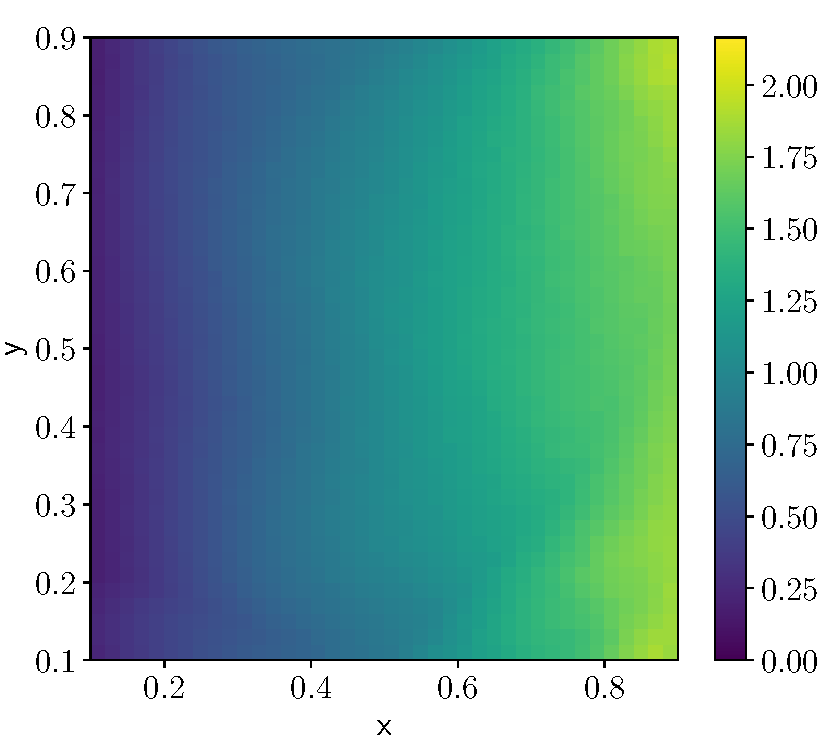
\includegraphics[width=0.32\textwidth, page=1]{./figures/bINN/linear_2dhists}
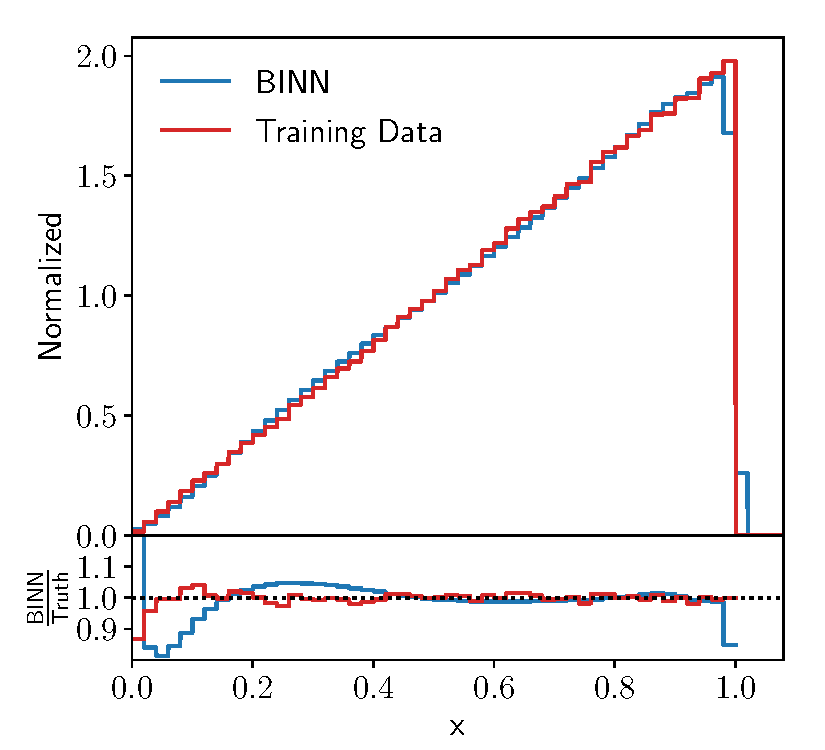
\includegraphics[width=0.32\textwidth, page=1]{./figures/bINN/linear_1dhists}
\includegraphics[width=0.32\textwidth, page=2]{./figures/bINN/linear_1dhists}
\caption{Two-dimensional and marginal densities for the linear wedge
  ramp.}
\label{fig:linear_ring_hists}
\end{figure}
%-------------------------------------------

In Fig.~\ref{fig:linear_unc} we include the predicted uncertainty
given by the BINN. For this purpose we train a network on the
two-dimensional parameter space and evaluate it for a set of points
with $x \in [0,1]$ and a constant $y$-value. In the left panel we
indicate the predicted uncertainty as an error bar around the density
estimate. Throughout the chapter we always remove the phase space
boundaries, because we observe that the model predicts there large 
uncertainties which would overall dominate the figures. The relative
uncertainty grows for small values of $x$ and hence small values of
$p(x,y)$, and it covers the deviation of the extracted density from
the true density well. These features are common to all our network
trainings. In the central and right panel of Fig.~\ref{fig:linear_unc}
we show the relative and absolute predicted uncertainties. The error
bar indicates how much $\sigma_\text{pred}$ varies for different
choices of $y$. We compute it as the standard deviation of different
values of $\sigma_\text{pred}$, after confirming that the central
values agrees within this range. As expected, the relative uncertainty
decreases towards larger $x$. However, the absolute uncertainty shows
a distinctive minimum in $\sigma_\text{pred}$ around $x \approx
0.45$. This minimum is a common feature in all our trainings, so we
need to explain it.

%-------------------------------------------
\begin{figure}[t]
\centering
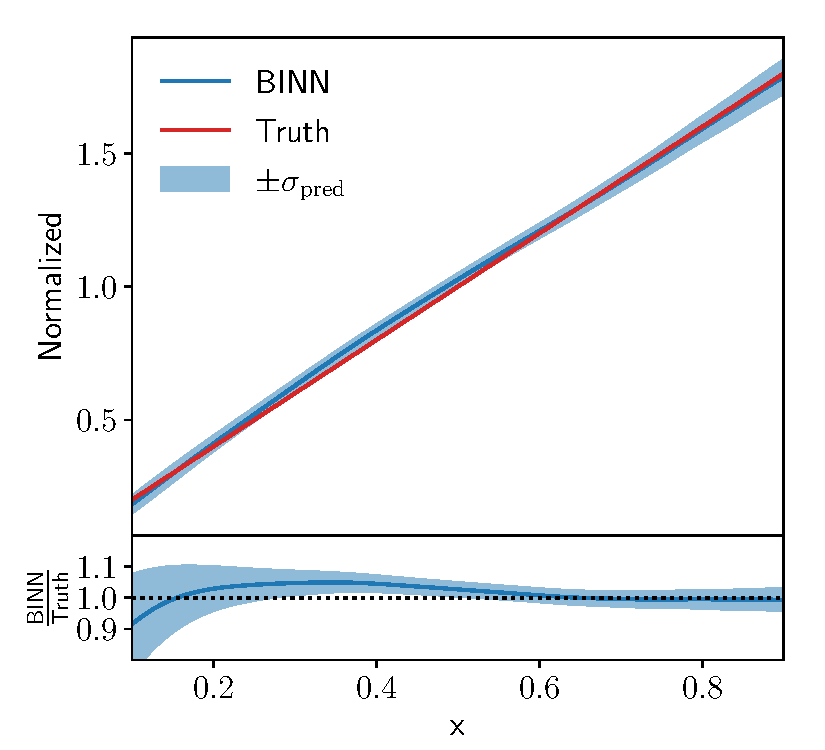
\includegraphics[width=0.32\textwidth, page=1]{./figures/bINN/linear_1dplots}
\includegraphics[width=0.32\textwidth, page=2]{./figures/bINN/linear_1dplots}
\includegraphics[width=0.32\textwidth, page=3]{./figures/bINN/linear_1dplots}
\caption{Density and predicted uncertainty distribution for the wedge
  ramp. In the left panel the density and uncertainty are averaged
  over several lines with constant $y$. In the central and right
  panels, the uncertainty band on $\sigma_\text{pred}$ is given by
  their variation.  The green curve represents a two-parameter fit to
  Eq.\eqref{eq:fit_wedge}.}
  \label{fig:linear_unc}
\end{figure}
%-------------------------------------------

To understand this non-trivial uncertainty distribution
$\sigma_\text{pred}(x)$ we focus on the non-trivial $x$-coordinate and
its linear behavior
%
\begin{align}
  p(x) = a  x + b
  \qquad \text{with} \qquad x \in [0,1] \; .
\end{align}
%
Because the network learns a normalized density, we can remove $b$ by
fixing the normalization,
%
\begin{align}
  p(x) = a \left( x - \frac{1}{2} \right) + 1 \; .
\end{align}
%
If we now assume that a network acts like a fit of $a$, , we can relate 
the uncertainty $\Delta a$ to an uncertainty in the density
%
\begin{align}
\sigma_\text{pred} \equiv \Delta p \approx \left| x - \frac{1}{2} \right| \; \Delta a \; .
\label{eq:simple_wedge}
\end{align}
%
The absolute value appears because the uncertainties are defined to be
positive, as encoded in the usual quadratic error propagation. The
uncertainty distribution has a minimum at $x=1/2$, close to the
observed value in Fig.~\ref{fig:linear_unc}.

The differences between the simple prediction in
Eq.\eqref{eq:simple_wedge} and our numerical findings in
Fig.~\ref{fig:linear_unc} is that the predicted uncertainty is not
symmetric and does not reach zero. To account for these sub-leading
effects we can expand our very simple ansatz to
%
\begin{align}
  p(x) = a  x + b
  \qquad \text{with} \qquad x \in [x_\text{min},x_\text{max}] \; .
\label{eq:fund_wedge}
\end{align}
%
Using the normalization condition we again remove $b$ and find
%
\begin{align}
  p(x)
  = a x
  +  \frac{ 1 - \frac{a}{2}(x_\text{max}^2 - x_\text{min}^2) }{ x_\text{max} - x_\text{min} } \; .
\end{align}
%
Again assuming a fit-like behaviour of the flow network we expect for
the predicted uncertainty
%
\begin{align}
\sigma_\text{pred}^2 \equiv (\Delta p)^2 =
    \left( x - \frac{1}{2} \right)^2 (\Delta a)^2
    + \left(1 + \frac{a}{2} \right)^2 (\Delta x_\text{max} )^2
    + \left(1 - \frac{a}{2} \right)^2 (\Delta x_\text{min} )^2 \; .
\label{eq:fit_wedge}
\end{align}
%
Adding $x_\text{max}$ adds an $x$-independent offset. Also accounting
for $x_\text{min}$ does not change the $x$-dependence of predicted
uncertainty. The slight shift of the minimum and the asymmetry between
the lower and upper boundaries in $x$ are not explained by this
argument.  We ascribe them to boundary effects, specifically the
challenge for the network to describe the correct approach towards
$p(x) \to 0$.

The green line in the lower panels of Fig.~\ref{fig:linear_unc} gives
a two-parameter fit of $\Delta a$ and $\Delta x_\text{max}$ to the
$\sigma_\text{pred}$ distribution from the BINN. It indicates that
there is a hierarchy in the way the network extracts the
$x$-independent term with high precision, whereas the uncertainty on
the slope $a$ is around 4\%.

%%%%%%%%%%%%%%%%%%%%%%%%%%%%%%%%%%%%%%%%%%%%%%%%%%%%%%%%%%%%%%%%%%%%%%%%
\subsection{Quadratic ramp}
\label{sec:toy_kicker}

%-------------------------------------------
\begin{figure}[b!]
\centering
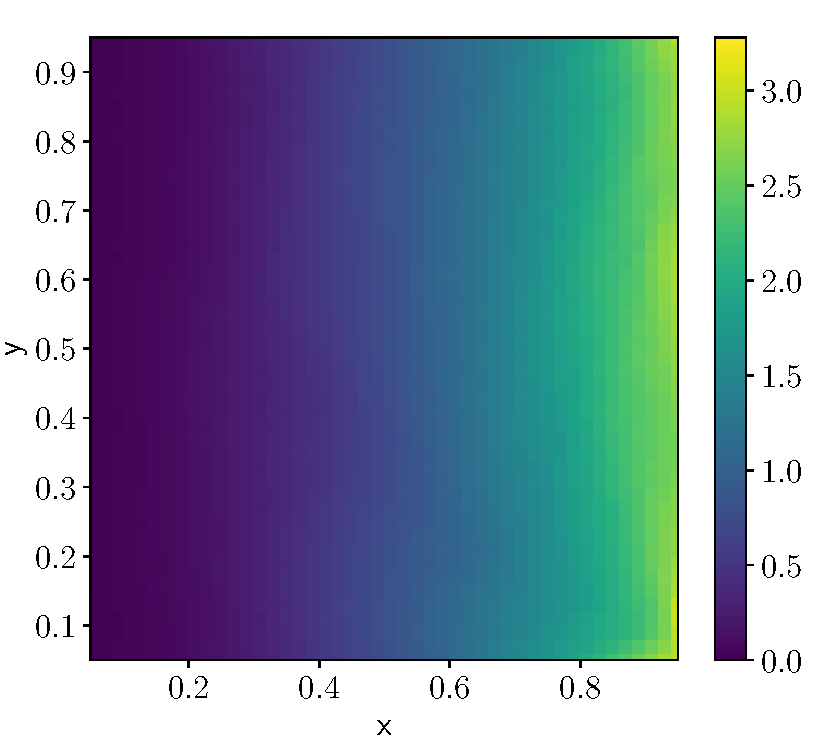
\includegraphics[width=0.32\textwidth, page=1]{./figures/bINN/quadratic_2dhists}
\includegraphics[width=0.32\textwidth, page=1]{./figures/bINN/quadratic_1dhists}
\includegraphics[width=0.32\textwidth, page=2]{./figures/bINN//quadratic_1dhists}
\caption{Two-dimensional and marginal densities for the quadratic ramp.}
\label{fig:quadratic_hists}
\end{figure}
%-------------------------------------------

We can test our findings from the linear wedge ramp using the slightly
more complex quadratic ramp,
%
\begin{align}
  p(x, y) =  \text{Quadr} (x\in[0,1]) \times \text{Const} (y \in[0, 1])
  = x^2 \times 3 \; .
%&= \frac{1}{2} \Theta [1 - x] \Theta [x + 1] \Theta[x + 0.5] \Theta[0.5 - x] \, \frac{1}{3} \left(x - \frac{1}{2} \right)^2
\label{eq:quadratic_dens}
\end{align}
%
We show the results from the network training for the density in
Fig.~\ref{fig:quadratic_hists} and find that the network describes the
density well, limited largely by the flat, low-statistics approach
towards the lower boundary with $p(x) \to 0$.

%-------------------------------------------
\begin{figure}[t]
\centering
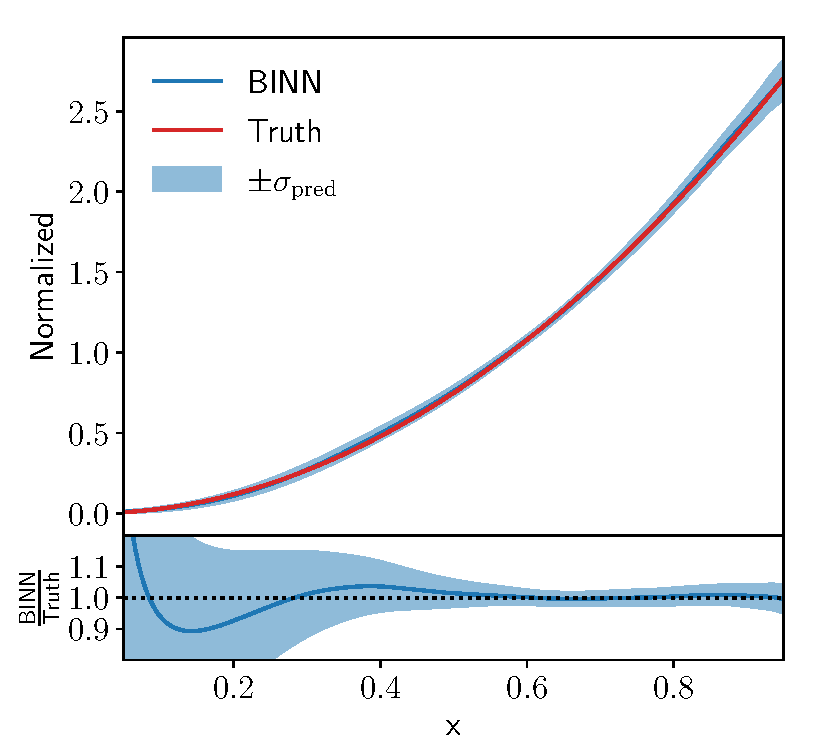
\includegraphics[width=0.32\textwidth, page=1]{./figures/bINN/quadratic_1dplots}
\includegraphics[width=0.32\textwidth, page=2]{./figures/bINN/quadratic_1dplots}
\includegraphics[width=0.32\textwidth, page=3]{./figures/bINN/quadratic_1dplots}
\caption{Density and predicted uncertainty distribution for the
  quadratic ramp. In the left panel the density and uncertainty are
  averaged over several lines with constant $y$. In the central and
  right panels, the uncertainty band on $\sigma_\text{pred}$ is given
  by their variation.  The green curve represents a two-parameter fit
  to Eq.\eqref{eq:fit_kicker}.}
\label{fig:quadratic_unc}
\end{figure}
%-------------------------------------------

In complete analogy to Fig.~\ref{fig:linear_unc} we show the complete
BINN output with the density $p(x,y)$ and the uncertainty
$\sigma_\text{pred}(x,y)$ in Fig.~\ref{fig:quadratic_unc}. As for the
linear case, the BINN reproduces the density well, deviations from the
truth being within the uncertainty in all points of phase
space. The indicated error bar on $\sigma_\text{pred}(x,y)$ is given by the
variation of the predictions for different $y$-values, after ensuring
that their central values agree.  The relative uncertainty at the
lower boundary $x = 0$ is large, reflecting the statistical limitation
of this phase-space region. An interesting feature appears again in
the absolute uncertainty, namely a maximum-minimum combination as a
function of $x$.

Again in analogy to Eq.\eqref{eq:fund_wedge} for the wedge ramp, we
start with the parametrization of the density
%
\begin{align}
  p(x) = a \, (x - x_0)^2
  \qquad \text{with} \qquad x \in [x_0, x_\text{max}] \; ,
\end{align}
%
where we assume that the lower boundary coincides with the minimum and
there is no constant offset. We choose to describe this density
through the minimum position $x_0$, coinciding the the lower end of
the $x$-range, and $x_\text{max}$ as the second parameter. The
parameter $a$ can be eliminated through the normalization condition
and we find
%
\begin{align}
  p(x)
%  =a \, (x - x_0)^2
  =3 \frac{(x - x_0)^2}{(x_\text{max} - x_0)^3} \; .
\end{align}
%
If we vary $x_0$ and $x_\text{max}$ we can trace two contributions to the
uncertainty in the density,
%
\begin{align}
\sigma_\text{pred} \equiv \Delta p
%&= \left| p \left( \frac{3}{x_\text{max} - x_0} - \frac{2}{x - x_0} \right) \right| \Delta x_0
%\notag \\
%&= \left| \frac{9 (x - x_0)^2}{(x_\text{max} - x_0)^4} - \frac{6 (x - x_0)}{(x_\text{max} - x_0)^3} \right| \Delta x_0
%\notag \\
%&= \frac{3}{(x_\text{max} - x_0)^4} \left| 3 (x - x_0)^2 - 2 (x - x_0) (x_\text{max} - x_0) \right| \Delta x_0
%\notag \\
%&= \frac{9}{(x_\text{max} - x_0)^4} \left| (x - x_0) \left( x - x_0 - \frac{2}{3} (x_\text{max} - x_0) \right) \right| \Delta x_0
%\notag \\
&\supset \frac{9}{(x_\text{max} - x_0)^4} \left| (x - x_0) \left( x - \frac{x_0}{3} - \frac{2 x_\text{max}}{3} \right) \right| \Delta x_0 \notag \\
\text{and} \qquad
\sigma_\text{pred} \equiv  \Delta p
%&= \left| p \; \frac{3}{x_\text{max} - x_0} \right| \Delta x_\text{max}
%\notag \\
%&= \left| 9 \frac{(x - x_0)^2}{(x_\text{max} - x_0)^4} \right| \Delta x_\text{max}
%\notag \\
&\supset \frac{9}{(x_\text{max} - x_0)^4} \; (x - x_0)^2 \; \Delta x_\text{max} \; ,
\label{eq:fit_kicker}
\end{align}
%
one from the variation of $x_0$ and one from the variation of
$x_\text{max}$. In analogy to Eq.\eqref{eq:fit_wedge} they need to be
added in quadrature.  If the uncertainty on $\Delta x_0$ dominates,
the uncertainty has a trivial minimum at $x=0$ and a non-trivial
minimum at $x=2/3$. From $\Delta x_\text{max}$ we get another
contribution which scales like $\Delta p \propto p(x)$. In
Fig.~\ref{fig:quadratic_unc} we clearly observe both contributions,
and the green line in the lower panels is given by the corresponding
2-parameter fig to the $\sigma_\text{pred}$ distribution from the
BINN.

%%%%%%%%%%%%%%%%%%%%%%%%%%%%%%%%%%%%%%%%%%%%%%%%%%%%%%%%%%%%%%%%%%%%%%%%
\subsection{Gaussian ring}
\label{sec:toy_ring}

%-------------------------------------------
\begin{figure}[b!]
\centering
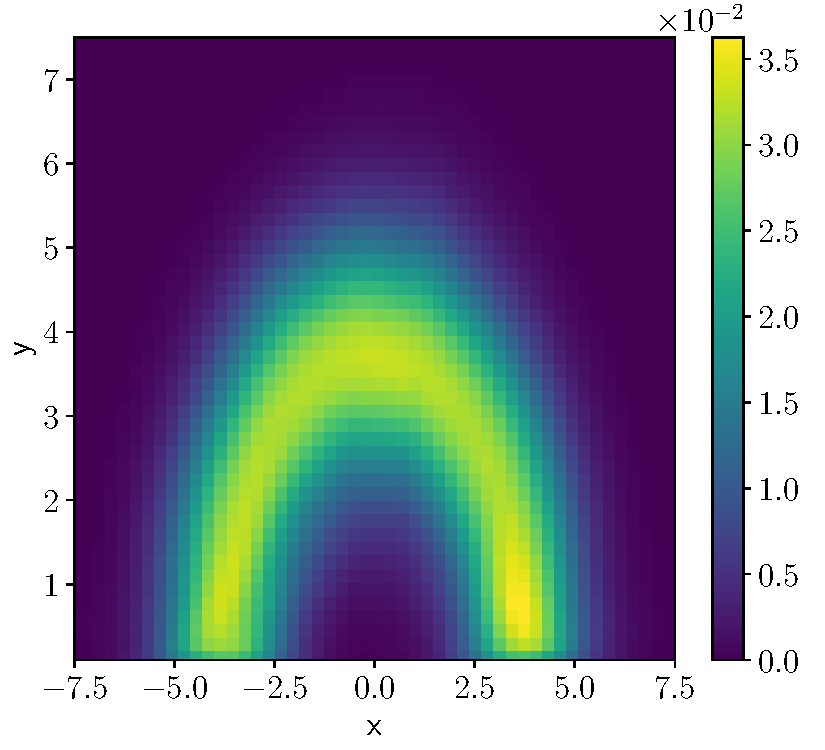
\includegraphics[width=0.32\textwidth, page=1]{./figures/bINN/gauss_ring_2dhists}
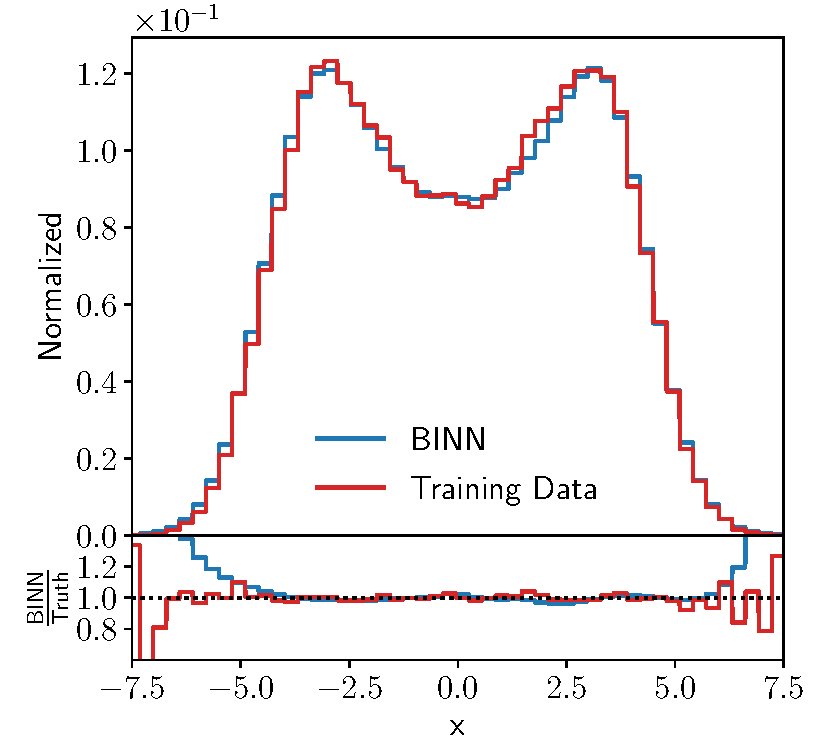
\includegraphics[width=0.32\textwidth, page=1]{./figures/bINN/gauss_ring_1dhists}
\includegraphics[width=0.32\textwidth, page=2]{./figures/bINN/gauss_ring_1dhists}
\caption{Two-dimensional and marginal densities for the Gaussian
  (half-)ring.}
\label{fig:gauss_hists}
\end{figure}
%-------------------------------------------

Our third example is a two dimensional Gaussian ring, which in terms
of polar coordinates reads
%
\begin{align}
p(r, \phi) = \text{Gauss}(r > 0; \mu=4, w=1) \times \text{Const}(\phi \in [0, \pi]) \; ,
\label{eq:gauss_dens}
\end{align}
%
We define the Gaussian density as the usual
%
\begin{align}
  \text{Gauss}(r)
&=  \frac{1}{\sqrt{2 \pi} \; w} \exp \left[ - \frac{1}{2 w^2} (r-\mu)^2 \right]
%  \notag \\
%  \text{Gauss}'(r) 
%&=  \frac{1}{\sqrt{2 \pi} \; w} \exp \left[ - \frac{1}{2 w^2} (r-\mu)^2 \right]
%  \frac{-1}{2w^2} ( 2r - 2\mu ) \notag \\
%&=\text{Gauss}(r) 
%  \; \frac{\mu-r}{w^2} 
\end{align}
%
The density defined in Eq.\eqref{eq:gauss_dens} can be translated into
Cartesian coordinates as
%
\begin{align}
p(x, y) = \text{Gauss}(r(x, y);\mu=4, w=1) \, \times \text{Const}(\phi(x, y) \in [0, \pi]) \times \dfrac{1}{r(x, y)}
\end{align}
%
where the additional factor $1/r$ comes from the Jacobian. We train
the BINN on Cartesian coordinates, just like in the two examples
before, and limit ourselves to $y>0$ to avoid problems induced by
learning a non-trivial topology in mapping the latent and phase
spaces.  In Fig.~\ref{fig:gauss_hists} we once again see that our
network describes the true two-dimensional density well.

%-------------------------------------------
\begin{figure}[t]
\centering
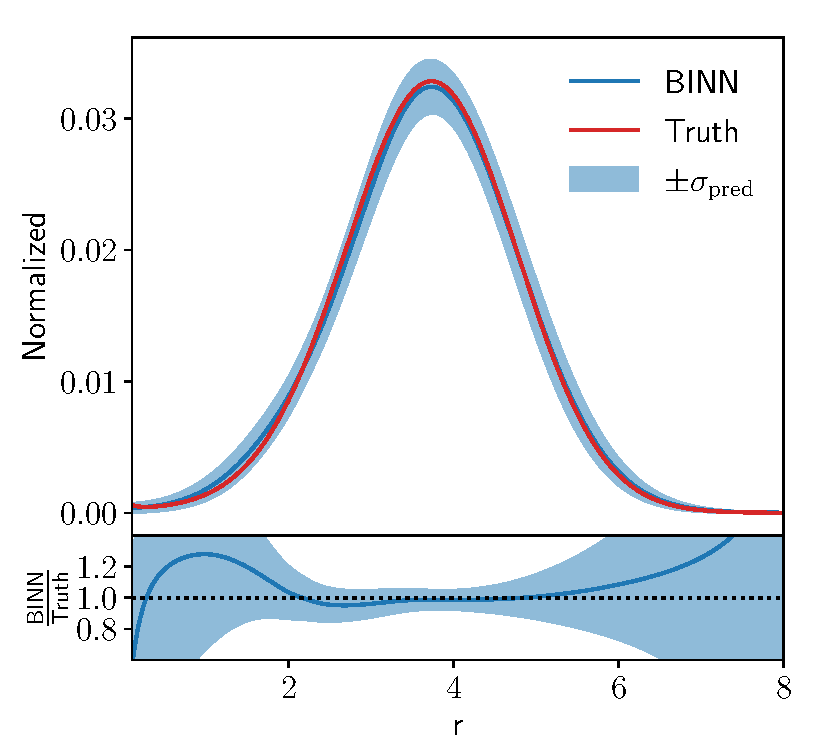
\includegraphics[width=0.32\textwidth, page=1]{./figures/bINN/gauss_ring_1dplots}
\includegraphics[width=0.32\textwidth, page=2]{./figures/bINN/gauss_ring_1dplots}
\includegraphics[width=0.32\textwidth, page=3]{./figures/bINN/gauss_ring_1dplots}
\caption{Cartesian density and predicted uncertainty distribution for
  the Gaussian ring. In the left panel the density and uncertainty are
  averaged over several lines with constant $\phi$. In the central and
  right panels, the uncertainty band on $\sigma_\text{pred}$ is given
  by their variation.  The green curve represents a two-parameter fit
  to Eq.\eqref{eq:gauss_fit}.}
\label{fig:gauss_unc}
\end{figure}
%-------------------------------------------

In Fig.~\ref{fig:gauss_unc} we show the Cartesian density but
evaluated on a line of constant angle. This form includes the Jacobian
and has the expected, slightly shifted peak position at $r_\text{max}
= 2 + \sqrt{3} = 3.73$. The BINN returns an uncertainty
which grows towards both boundaries.  The error band easily covers the
deviation of the density learned by the BINN and the true
density. While the relative predicted uncertainty appears to have a
simple minimum around the peak of the density, we again see that the
absolute uncertainty has a distinct structure with a local minimum
right at the peak. The question is what we can learn about the INN
from this pattern in the BINN.

As before, we describe our distribution in the relevant direction in
terms of convenient fit parameters. For the Gaussian radial density
these are the mean $\mu$ and the width $w$ used in
Eq.\eqref{eq:gauss_dens}. The contributions driven by the extraction
of the mean in Cartesian coordinates reads
%
\begin{align}
\sigma_\text{pred} &\equiv  \Delta p \supset
%  \Bigr| \dfrac{d}{d \mu} \, p(x, y | \mu) \Bigr|_{\mu=4}  \, \Delta \mu  \Bigr| \\
% &= \Bigr| \frac{d}{d \mu} \, G(r(x, y) | \mu, \sigma=1) \, \dfrac{1}{r(x, y)} \Bigr|_{\mu=4} \, \Delta \mu \Bigr|\\
\left| \frac{G(r)}{r} \, \frac{\mu - r}{w^2} \right| \Delta \mu
\notag \\
\text{and} \qquad
\sigma_\text{pred} &\equiv \Delta p \supset
\left| \frac{(r - \mu)^2}{w^3} - \frac{1}{w} \right| \Delta w \; .
%\notag \\
%&= \left| \frac{(r - \mu)^2 - w^2}{w^3} \right| \Delta w 
%\notag \\
%&= \left| \frac{r^2 - 2 \mu r + \mu^2 - w^2}{w^3} \right| \Delta w 
%\notag \\
\label{eq:gauss_fit}
\end{align}
%
In analogy to Eq.\eqref{eq:fit_wedge} the two contributions need to be
added in quadrature for the full, fit-like uncertainty.  The
contribution from the the mean has a minimum at $r=\mu=4$ and is
otherwise dominated by the exponential behavior of the Gaussian, just
as we observe in the BINN result.  In the opposite limit of $\Delta
\mu \ll \Delta w$ the uncertainty develops the maxima at $r=3$ and
$r=5$, which we observe in Fig.~\ref{fig:gauss_unc}. In the central and right 
panels we show a one-parameter fit of the BINN output and find that the 
network determined the mean of the Gaussian as $\mu = 4 \pm 0.037$. 
We observe that including $\Delta w$ does not improve the goodness of the fit.

%%%%%%%%%%%%%%%%%%%%%%%%%%%%%%%%%%%%%%%%%%%%%%%%%%%%%%%%%%%%%%%%%%%%%%%%
\subsection{Errors vs training statistics}
\label{sec:toy_stats}

%-------------------------------------------
\begin{figure}[t]
\centering
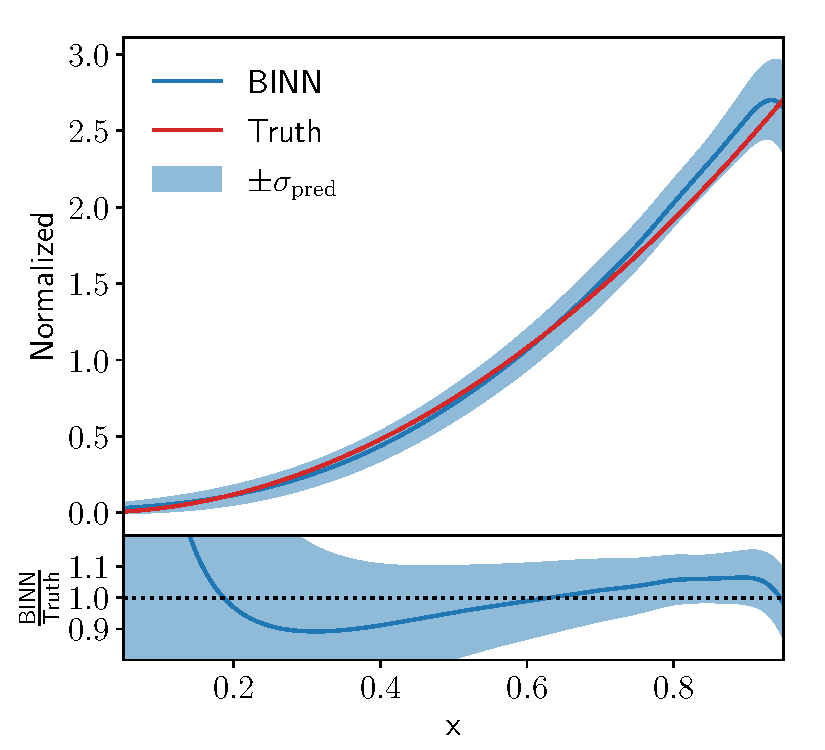
\includegraphics[width=0.32\textwidth, page=1]{./figures/bINN/training_size_10k}
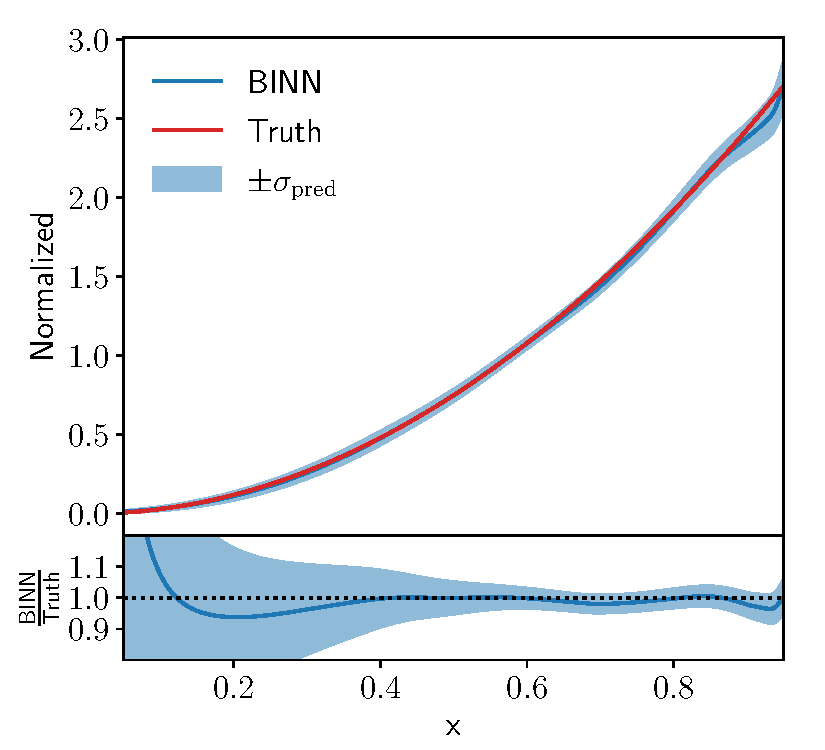
\includegraphics[width=0.32\textwidth, page=1]{./figures/bINN/training_size_100k}
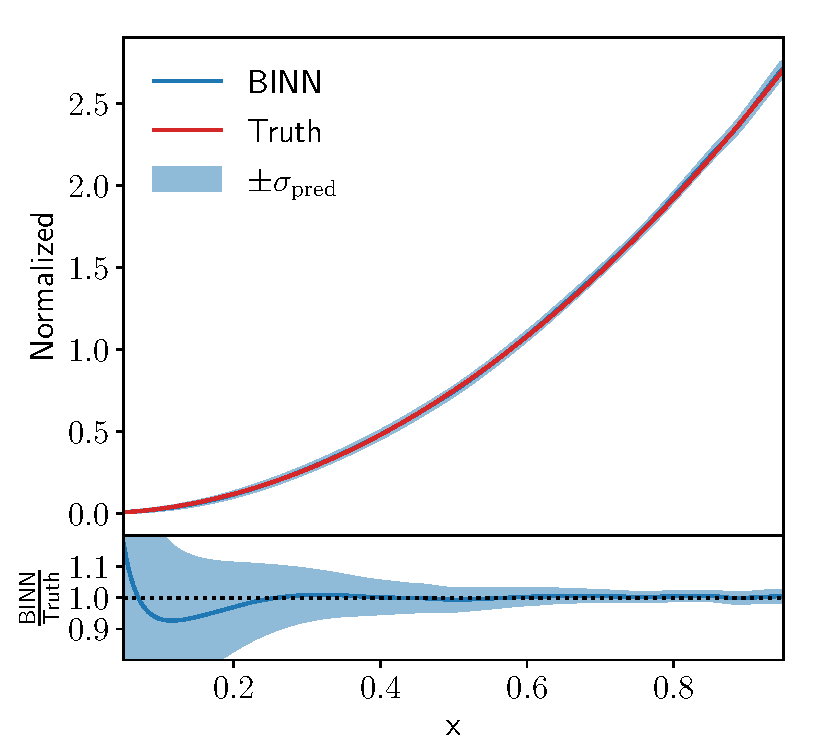
\includegraphics[width=0.32\textwidth, page=1]{./figures/bINN/training_size_1M} \\
\includegraphics[width=0.32\textwidth, page=2]{./figures/bINN/training_size_10k}
\includegraphics[width=0.32\textwidth, page=2]{./figures/bINN/training_size_100k}
\includegraphics[width=0.32\textwidth, page=2]{./figures/bINN/training_size_1M}
\caption{Dependence of the density (upper) and absolute
  uncertainty (lower) on the training statistics for the quadratic ramp. We illustrate BINNs trained
  on 10k, 100k, and 1M events (left to right), to be compared to 300k
  events used for Fig.~\ref{fig:quadratic_unc}. Our training routine
  ensures that all models receive the same number of weights updates,
  regardless of the training set size.}
\label{fig:training_size}
\end{figure}
%-------------------------------------------

Even though it is clear from the above discussion that we cannot
expect the predicted uncertainties to have a simple scaling pattern,
like for the regression~\cite{Kasieczka:2020vlh} and
classification~\cite{Bollweg:2019skg} networks, there still remains
the question of how the BINN uncertainties change with the size of the
training sample.

In Fig.~\ref{fig:training_size} we show how the BINN predictions for
the density and uncertainty change if we vary the training sample size
from 10k events to 1M training events. Note that for all toy
models, including the quadratic ramp in Sec.~\ref{sec:toy_kicker}, we use
300k training events. For the small 10k training sample, we see that
the instability of the BINN density becomes visible even for our
reduced $x$-range.  The peak-dip pattern of the absolute uncertainty,
characteristic for the quadratic ramp, is also hardly visible, indicating
that the network has not learned the density well enough to determine
its shape. Finally, the variation of the predicted density explodes
for $x>0.4$, confirming the picture of a poorly trained model. As a
rough estimate, the absolute uncertainty at $x=0.5$ with a density
value $p(x,y) = 0.75$ ranges around $\sigma_\text{pred} =
0.11~...~0.15$.

For 100k training events we see that the patterns discussed in
Sec.~\ref{sec:toy_kicker} begin to form. The density and uncertainty
encoded in the network are stable, and the peak-dip with a minimum
around $x=2/3$ becomes visible. As a rough estimate we can read off
$\sigma_\text{pred}(0.5) \approx 0.06 \pm 0.03$. For 1M training
events the picture improves even more and the network extracts a
stable uncertainty of $\sigma_\text{pred}(0.5) \approx 0.03 \pm
0.01$. Crucially, the dip around $x \approx 2/3$ remains, and even
compared to Fig.~\ref{fig:quadratic_unc} with its 300k training events
the density and uncertainty at the upper phase space boundary are much
better controlled.

Finally, we briefly comment on a frequentist interpretation of the
BINN output. We know from simpler Bayesian 
networks~\cite{Bollweg:2019skg,Kasieczka:2020vlh}
that it is possible to reproduce the predicted uncertainty using
an ensemble of deterministic networks with the same architecture.
However, from those studies we also know that our class of Bayesian
networks has a very efficient built-in regularization, so
this kind of comparison is not trivial. For the BINN results shown
in this chapter we find that the detailed patterns in the
absolute uncertainties are extracted by the Bayesian network much more
effectively than they would be for ensembles of deterministic INNs.
For naive implementations with a similar network size and no fine-tuned
regularization these patterns are somewhat harder to extract. On the
other hand, in stable regions without distinctive patterns
the spread of ensembles of deterministic networks
reproduces the predicted uncertainty reported by the BINN.

%%%%%%%%%%%%%%%%%%%%%%%%%%%%%%%%%%%%%%%%%%%%%%%%%%%%%%%%%%%%%%%%%%%%%%%%
\subsection{Marginalizing phase space}
\label{sec:toy_marginal}

Before we move to a more LHC-related problem, we need to study how the
BINN provides uncertainties for marginalized kinematic
distributions. In all three toy examples the two-dimensional phase
space consists of one physical and one trivial direction. For
instance, the quadratic ramp in Sec.~\ref{sec:toy_kicker} has a quadratic
physical direction, and in a typical phase space problem we would
integrate out the trivial, constant direction and show a
one-dimensional kinematic distribution. From our effectively
one-dimensional uncertainty extraction we know that the absolute
uncertainty has a characteristic maximum-minimum combination, as seen
in the lower-right panel of Fig.~\ref{fig:quadratic_unc}.

To compute the uncertainty for a properly marginalized phase space
direction, we remind ourselves how the BINN computes the density and
the predicted uncertainty by sampling over the weights,
%
\begin{align}
p(x, y) &= \int d\theta \, q(\theta) \, p(x, y | \theta)  \notag \\
\sigma_\text{pred}^2(x, y) &= \int d\theta \, q(\theta) \left[ p(x, y | \theta) - p(x, y) \right]^2 \, .
\label{eq:sigma_pred}
\end{align}
%
If we integrate over the $y$-direction, the marginalized density is
defined as
%
\begin{align}
  p(x)  = \int dy \, p(x,y)
       =& \int dy d\theta \, q(\theta) \, p(x, y | \theta)  \notag \\
       =& \int d\theta \, q(\theta) \, \int dy \, p(x, y | \theta)
       \equiv \int d\theta \, q(\theta) \, p(x | \theta) \; ,
\label{eq:p_marginal}
\end{align}
%
which implicitly defines $p(x|\theta)$ in the last step, notably
without providing us with a way to extract it in a closed form. The
key step in this definition is that we exchange the order of the $y$
and $\theta$ integrations. Nevertheless, with this definition at hand,
we can \textsl{define} the uncertainty on the marginalized
distribution as
%
\begin{align}
  \sigma_\text{pred}^2 (x) = \int d\theta \, q(\theta) \left[ p(x | \theta) - p(x) \right]^2 \; .
\label{eq:sigma_pred_marg}
\end{align}
%
We illustrate this construction with a trivial $p(x,y) = p(x,y_0)$,
where we can replace the trivial $y$-dependence by a fixed choice
$y=y_0$ just like for the wedge and quadratic ramps. Here we find, modulo
a normalization constant in the $y$-integration
%
\begin{align}
  \sigma_\text{pred}^2 (x)
  &= \int d\theta \, q(\theta) \left[ p(x | \theta) - p(x) \right]^2
  \notag \\
  &= \int d\theta \, q(\theta) \int dy \; \left[ p(x,y_0 | \theta) - p(x,y_0) \right]^2
  \notag \\
  &= \int dy d\theta \, q(\theta) \; \left[ p(x,y_0 | \theta) - p(x,y_0) \right]^2
   = \int dy \, \sigma_\text{pred}^2 (x,y_0) = \sigma_\text{pred}^2 (x,y_0) \; .
\end{align}
%
Adding a trivial $y$-direction does not affect the predicted
uncertainty in the physical $x$-direction.

%-------------------------------------------
\begin{figure}[t]
\centering
\includegraphics[width=0.32\textwidth,page=3]{./figures/bINN/quadratic_1dhists_with_unc}
\hspace*{0.1\textwidth}
\includegraphics[width=0.32\textwidth,page=4]{./figures/bINN/quadratic_1dhists_with_unc}\\
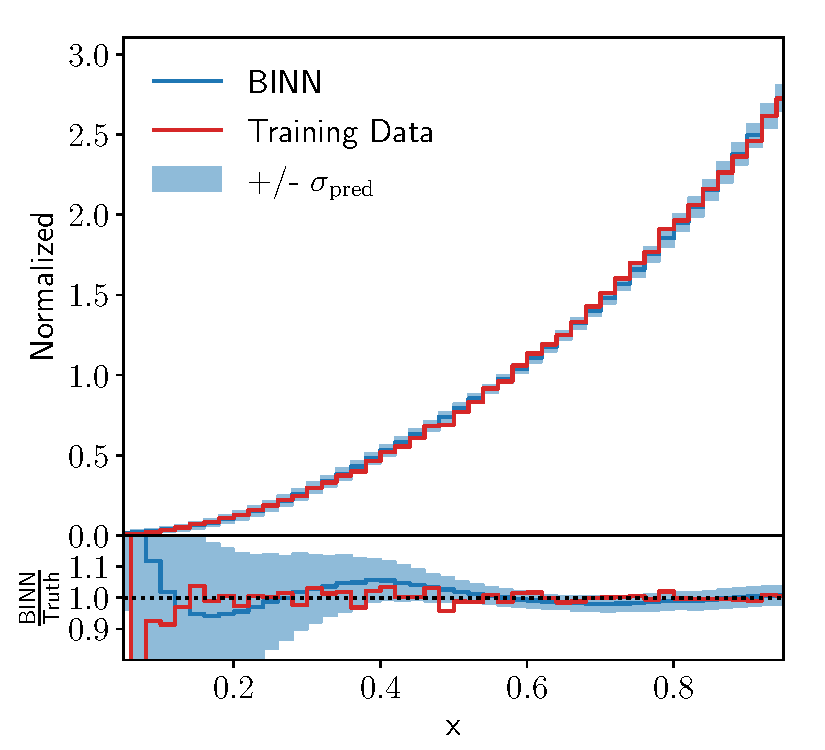
\includegraphics[width=0.32\textwidth,page=1]{./figures/bINN/quadratic_1dhists_with_unc}
\hspace*{0.1\textwidth}
\includegraphics[width=0.32\textwidth,page=2]{./figures/bINN/quadratic_1dhists_with_unc}
\caption{Marginalized densities and predicted uncertainties for the
  quadratic ramp. Instead of the true distribution we now show the training data as a reference, to illustrate possible limitations. We use 10M phase space point to guarantee a stable prediction.}
\label{fig:marginalized}
\end{figure}
%-------------------------------------------

As mentioned above, unlike for the joint density, $p(x, y | \theta)$
we do not know the closed form of the marginal distributions $p(x)$ or
$p(x| \theta)$. Instead, we can approximate the marginalized
uncertainties through a combined sampling in $y$ and $\theta$.  We
start with one set of weights $\theta_i$ from the weight
distributions, based on one random number per INN weight. We now
sample $N$ points in the latent space, $z_j$, and compute $N$ phase
space point $x_j$ using the BINN configuration $\theta_i$. We then bin
the wanted phase space direction $x$ and approximate $p(x|\theta_i)$
by a histogram. We repeat this procedure $i=1~...~M$ times to extract
$M$ histograms with identical binning. This allows us to compute a
mean and a standard deviation from $M$ histograms to approximates
$p(x)$ and $\sigma_\text{pred}(x)$. The approximation of
$\sigma_\text{pred}$ should be an over-estimate, because it includes
the statistical uncertainty related to a finite number of samples per
bin.  For $N \gg 1$ this contribution should become negligible. With
this procedure we effectively sample $N \times M$ points in phase
space.

Following Eq.\eqref{eq:p_marginal}, we can also fix the phase space
points, so instead of sampling for each weight sample another set of
phase space points, we use the same phase space points for each weight
sampling. This should stabilize the statistical fluctuations, but with
the drawback of relying only on an effective number of $N$ phase space
points. Both approaches lead to the same $\sigma_\text{pred}$ for
sufficiently large $N$, which we typically set to $10^5~...~10^6$. For
the Bayesian weights we find stable results for $M=30~...~50$.

In Fig.~\ref{fig:marginalized} we show the marginalized densities and
predicted uncertainties for the quadratic ramp.  In $y$-direction the
density and the predicted uncertainty show the expected flat
behaviour. The only exception are the phase space boundaries, where the
density starts to deviate slightly from the training data and the
uncertainty correctly reflects that instability.  In $x$-direction,
the marginalized density and uncertainty can be compared to their
one-dimensional counterparts in Fig.\ref{fig:quadratic_unc}. While we
expect the same peak-dip structure, the key question is if the
numerical values for $\sigma_\text{pred}(x)$ change. If the network
learns the $y$-direction as uncorrelated additional data, the
marginalized uncertainty should decrease through a larger effective
training sample. This is what we typically see for Monte Carlo
simulations, where a combination of bins in an unobserved directions
leads to the usual reduced statistical uncertainty. On the other hand,
if the network learns that the $y$-directions is flat, then adding
events in this direction will have no effect on the uncertainty of the
marginalized distribution. This would correspond to a set of fully
correlated bins, where a combination will not lead to any improvement
in the uncertainty. In Fig.~\ref{fig:marginalized} we see that the
$\sigma_\text{pred}(x)$ values on the peak, in the dip, and to the
upper end of the phase space boundary hardly change from the
one-dimensional results in Fig.\ref{fig:quadratic_unc}. This strengthens
our general observation, that the (B)INN learns a functional form of
the density in both directions, in close analogy to a fit. It also
means that the uncertainty from the generative network training is not
described by the simple statistical scaling we observed for simpler
models~\cite{Bollweg:2019skg,Kasieczka:2020vlh}.

%%%%%%%%%%%%%%%%%%%%%%%%%%%%%%%%%%%%%%%%%%%%%%%%%%%%%%%%%%%%%%%%%%%%%%%%
\section{LHC events with uncertainties}
\label{sec:lhc}

%----------------------------------------------------------
\begin{table}[b!]
\begin{small} \begin{center}
\begin{tabular}{l r }
\toprule
Parameter & Flow \\
\midrule
Hidden layers (per block) & 2\\
Units per hidden layer & 64\\
Batch size & 512 \\
Epochs & 500 \\
Trainable weights & $\sim$ 182k \\
Number of training events & $\sim$ 1M\\
Optimizer & Adam\\
($\alpha$, $\beta_1$, $\beta_2$)  & ($1\times10^{-3}$, 0.9, 0.999) \\
Coupling layers & 20 \\
Prior width & 1 \\
\bottomrule
\end{tabular}
\end{center} \end{small}
\caption{Hyper-parameters for the Drell-Yan data set, implemented in
  pytorch(v1.4.0)~\cite{pytorch}.}
\label{tab:DY_param_details}
\end{table}
%----------------------------------------------------------

As a physics example we consider the Drell-Yan process
%
\begin{align}
pp \rightarrow Z \rightarrow e^+ e^- \; ,
\end{align}
%
with its simple $2 \to 2$ phase space combined with the parton
density. The training set consists of an unweighted set of 4-vectors
simulated with madgraph~\cite{madgraph} at 13~TeV collider energy
with the NNPDF2.3 parton densities~\cite{Ball:2013hta}. We fix the
masses of the final-state leptons and enforce momentum conservation in
the transverse direction, which leaves us with a four-dimensional
phase space. In our discussion we limit ourselves to a sufficiently
large set of one-dimensional distributions. For these marginalized
uncertainties we follow the procedure laid out in
Sec.~\ref{sec:toy_marginal} with 50 samples in the BINN-weight
space. In Tab.~\ref{tab:DY_param_details} we give the relevant
hyper-parameters for this section.


%----------------------------------------------------------
\begin{figure}[t]
\includegraphics[width=0.32\textwidth, page=1]{./figures/bINN/DrellYan_without_mmd_1dhists}
\includegraphics[width=0.32\textwidth, page=3]{./figures/bINN/DrellYan_without_mmd_1dhists}
\includegraphics[width=0.32\textwidth, page=21]{./figures/bINN/DrellYan_without_mmd_1dhists}\\
\includegraphics[width=0.32\textwidth, page=7]{./figures/bINN/DrellYan_without_mmd_1dhists}
\includegraphics[width=0.32\textwidth, page=25]{./figures/bINN/DrellYan_without_mmd_1dhists}
\includegraphics[width=0.32\textwidth, page=27]{./figures/bINN/DrellYan_without_mmd_1dhists}
\caption{One-dimensional (marginalized) kinematic distributions for
  the Drell-Yan process.  We show the central prediction from the BINN
  and include the predicted uncertainty from the BINN as the blue
  band. The red band indicates the statistical uncertainty of the
  training data per bin in the Gaussian limit.}
\label{fig:DY}
\end{figure}
%----------------------------------------------------------

%----------------------------------------------------------
\begin{figure}[t]
\includegraphics[width=0.32\textwidth, page=2]{./figures/bINN/DrellYan_without_mmd_1dhists}
\includegraphics[width=0.32\textwidth, page=4]{./figures/bINN/DrellYan_without_mmd_1dhists}
\includegraphics[width=0.32\textwidth, page=22]{./figures/bINN/DrellYan_without_mmd_1dhists}\\
\includegraphics[width=0.32\textwidth, page=8]{./figures/bINN/DrellYan_without_mmd_1dhists}
\includegraphics[width=0.32\textwidth, page=26]{./figures/bINN/DrellYan_without_mmd_1dhists}
\includegraphics[width=0.32\textwidth, page=28]{./figures/bINN/DrellYan_without_mmd_1dhists}
\caption{Absolute and relative uncertainties as a function of some of
  the kinematic Drell-Yan observables shown in Fig.~\ref{fig:DY}.}
\label{fig:DY_unc}
\end{figure}
%----------------------------------------------------------

To begin with, we show a set of generated kinematic distributions in
Fig.~\ref{fig:DY}. The positron energy features the expected strong
peak from the $Z$-resonance. Its sizeable tail to larger energies is
well described by the training data to $E_e \approx 280$~GeV. The
central value learned by the BINN becomes unstable at slightly lower
values of 250~GeV, as expected. The momentum component $p_x$ is not
observable given the azimuthal symmetry of the detector, but it's
broad distribution is nevertheless reproduced correctly. The
predicted uncertainty covers the slight deviations over the entire
range. What is observable at the LHC is the transverse momentum of the
outgoing leptons, with a similar distribution as the energy, just with
the $Z$-mass peak at the upper end of the distribution. Again, the
predicted uncertainty determined by the BINN covers the slight
deviations from the truth on the pole and in both tails. In the second
row we show the $p_z$ component as an example for a strongly peaked
distribution, similar to the Gaussian toy model in
Sec.~\ref{sec:toy_ring}.

While the energy of the lepton pair has a similar basic form as the
individual energies, we also show the invariant mass of the
electron-positron pair, which is described by the usual Breit-Wigner
peak. It is well known that this intermediate resonance is especially
hard to learn for a network, because it forms a narrow, highly
correlated phase space structure. Going beyond the precision shown
here would for instance require an additional MMD loss, as described
 in Ref.~\cite{fcgan}.
This resonance peak is the only distribution, where the predicted
uncertainty does not cover the deviation of the BINN density from the
truth. This apparent failure corresponds to the fact that generative
networks always overestimate the width and hence underestimate the
height of this mass peak~\cite{gan_phasespace}.  This is an example of
the network being limited by the expressive power in phase space
resolution, generating an uncertainty which the Bayesian version
cannot account for.

In Fig.~\ref{fig:DY_unc} we show a set of absolute and relative
uncertainties from the BINN. The strong peak combined with a narrow
tail in the $E_e$ distribution shows two interesting features. Just
above the peak the absolute uncertainty drops more rapidly than
expected, a feature shared by the wedge and quadratic ramps at their
respective upper phase space boundaries. The shoulder around $E_e
\approx 280$~GeV indicates that for a while the predicted uncertainty
follows the increasingly poor modelling of the phase space density by
the BINN, to a point where the network stops following the truth curve
altogether and the predicted uncertainty is limited by the expressive
power of the network.  Unlike the absolute uncertainty, the relative
uncertainty keeps growing for increasing values of $E_e$.  This
behavior illustrates that in phase space regions where the BINN starts
failing altogether, we cannot trust the predicted uncertainty either,
but we see a pattern in the intermediate phase space regime where the
network starts failing.

The second kinematic quantity we select is the
$x$-component of the momentum, which forms a relative flat central
plateau with sharp cliffs at each side. Any network will have trouble
learning the exact shape of such sharp phase space patterns. Here the
BINN keeps track of this, the absolute and the relative
uncertainties indeed explode. The only difference between the two is
that the density at the foot of the plateau drops even
faster than the learned absolute uncertainty, so their ratio keeps
growing.

Finally, we show the result for the Breit-Wigner mass peak, the
physical counterpart of the Gaussian ring model of
Sec.~\ref{sec:toy_ring}. Indeed, we see exactly the same pattern,
namely a distinctive minimum in the predicted uncertainty right on
the mass peak.  This pattern can be explained by the network learning
the general form of a mass peak and then adjusting the mean and the
width of this peak. Learning the peak position leads to a minimum of
the uncertainty right at the peak, and learning the width brings up
two maxima on the shoulders of the mass peak.  In combination
Fig.~\ref{fig:DY} and \ref{fig:DY_unc} show that the BINN
traces uncertainties in generated LHC events just as for the toy
models.

%%%%%%%%%%%%%%%%%%%%%%%%%%%%%%%%%%%%%%%%%%%%%%%%%%%%%%%%%%%%%%%%%%%%%%%%
\section{Conclusions and outlook}

Controlling the output of generative networks and quantifying their
uncertainties is the main task for any application in LHC physics, be
it in forward generation, inversion, or inference.  We have proposed
to use a Bayesian invertible network (BINN) to quantify the
uncertainties from the network training for each generated event. For
a series of two-dimensional toy models and an LHC-inspired
application we have shown how the Bayesian setup indeed generates an
uncertainty distribution, over the full phase space and over marginalized phase
spaces. As expected, the learned uncertainty shrinks with an improved training
statistics. Our method can be trivially extended
from unweighted to weighted events by adapting the simple MLE loss.
An intriguing result from our study is that the combined learning of
the density and uncertainty distributions allows us to draw conclusions on
how a normalizing-flow network like the BINN learns a distribution. 
We find that the uncertainty distributions are naturally explained by a
fit-like behavior of the network, rather than a patch-wise learning of
the density. For the LHC, this can be seen for instance in the
non-trivial uncertainty for an intermediate Breit-Wigner
resonance. 

%\end{document}
